\documentclass[onecolumn, draftclsnofoot,10pt, compsoc]{IEEEtran}
\usepackage{graphicx}
\usepackage{url}
\usepackage{setspace}

\usepackage{geometry}
\geometry{textheight=9.5in, textwidth=7in}

% 1. Fill in these details
\def \CapstoneTeamName{Education Simulations}
\def \CapstoneTeamNumber{53}
\def \GroupMemberOne{Cameron Friel}
\def \GroupMemberTwo{Kelli Ann Ulep}
\def \GroupMemberThree{Samuel Wilson}
\def \CapstoneProjectName{Interactive 2D simulations to support Inquiry-Based Learning in Mechanical Engineering}
\def \CapstoneSponsorCompany{Oregon State University, School of Chemical, Biological, and Environmental Engineering}
\def \CapstoneSponsorPersonOne{Milo Koretsky}
\def \CapstoneSponsorPersonTwo{Tom Ekstedt}


% 2. Uncomment the appropriate line below so that the document type works
\def \DocType{		%Problem Statement
				Requirements Document
				%Technology Review
				%Design Document
				%Progress Report
				}
			
\newcommand{\NameSigPair}[1]{\par
\makebox[2.75in][r]{#1} \hfil 	\makebox[3.25in]{\makebox[2.25in]{\hrulefill} \hfill		\makebox[.75in]{\hrulefill}}
\par\vspace{-12pt} \textit{\tiny\noindent
\makebox[2.75in]{} \hfil		\makebox[3.25in]{\makebox[2.25in][r]{Signature} \hfill	\makebox[.75in][r]{Date}}}}
% 3. If the document is not to be signed, uncomment the RENEWcommand below
%\renewcommand{\NameSigPair}[1]{#1}

%%%%%%%%%%%%%%%%%%%%%%%%%%%%%%%%%%%%%%%
\begin{document}
\begin{titlepage}
    \pagenumbering{gobble}
    \begin{singlespace}
    	
\includegraphics[height=4cm]{coe_v_spot1}
        \hfill 
        % 4. If you have a logo, use this includegraphics command to put it on the coversheet.
        %\includegraphics[height=4cm]{CompanyLogo}   
        \par\vspace{.2in}
        \centering
        \scshape{
            \huge CS Capstone \DocType \par
            {\large\today}\par
            \vspace{.5in}
            \textbf{\Huge\CapstoneProjectName}\par
            \vfill
            {\large Prepared for}\par
            \Huge \CapstoneSponsorCompany\par
            \vspace{5pt}
            {\Large
                \NameSigPair{\CapstoneSponsorPersonOne}\par
                \NameSigPair{\CapstoneSponsorPersonTwo}\par
            }
            {\large Prepared by }\par
            Group\CapstoneTeamNumber\par
            % 5. comment out the line below this one if you do not wish to name your team
            \CapstoneTeamName\par 
            \vspace{5pt}
            {\Large
                \NameSigPair{\GroupMemberOne}\par
                \NameSigPair{\GroupMemberTwo}\par
                \NameSigPair{\GroupMemberThree}\par
            }
            \vspace{20pt}
        }
        \begin{abstract}
        % 6. Fill in your abstract    
This project involves solving the problem of some universities lacking resources to visually show physical and mechanical interactions for Mechanical Engineering concepts in the classroom.
This project is built on the research that shows that students can achieve a better understanding of difficult concepts by learning through simulated environments that they can interact with.
By implementing 2D simulations based on these concepts, students will be able to visually interpret the concepts in the course.
The goal of this document is to set the requirements for these 2D simulations, listing all the features which shall be expected for this project.
        \end{abstract}     
    \end{singlespace}
\end{titlepage}
\newpage
\pagenumbering{arabic}
\tableofcontents
% 7. uncomment this (if applicable). Consider adding a page break.
%\listoffigures
%\listoftables
\clearpage

% 8. now you write!
\section{Introduction}
\subsection{Purpose}
The purpose of this document is to present the requirements for the Interactive 2D simulations to support Inquiry-Based Learning in Mechanical Engineering project, as well as expand on the intent behind the project. This document is intended to be read by the clients of the project, as well as the projects team members in order to bind the two parties to a contract regarding the requirements of the project.
\subsection{Scope}
Our product will consist of six variations of a two dimensional simulation based on mechanical engineering concepts in order to support inquiry based learning for mechanical engineering students. The simulations will be hosted on the Concept Warehouse website, which is a website that provides interactive learning opportunities for classrooms. While the simulation is running, real time mathematical feedback will be provided in the form of graphs or simply values in the simulation. There will be start/stop, and reset button within each simulation so that the student can explore the simulations as many times or at as many points as they need to. The students will also be able to modify specific parameters within the simulations in the sixth variation of the simulation, such as mass, friction, and angles.
\subsection{Product overview}
This document contains two more sections. The second section provides an overarching description of the product. The third section contains the specific requirements for the project.
\section{Overall Description}
\subsection{Product perspective}
Our product is part of a larger system, that being the Concept Warehouse, so students will need to click on a hyperlink within the Concept Warehouse website in order to navigate to our product. Each simulation will be powered by a 2D physics engine on a standalone web page. Each web page will have a canvas window to the left hand portion of the screen where the simulation will occur. Below the canvas will live buttons to start, stop, and restart the simulation. On the right side of the canvas will be parameter fields a student could interact with to change the way the simulation interacts. Above the parameter fields will be live mathematical feedback showing the student how the different parameters are changing during the simulation.
\subsection{User characteristics}
Our product is intended to be used by mechanical engineering students whose college is subscribed to the Concept Warehouse.
\subsection{Limitations}
Our product will need to be able to run on all modern web browsers, such as Chrome, Safari, and Firefox. A high quality camera might also be needed to record a live demonstration of the simulations to be embedded within the web page.
\section{Specific Requirements}
\subsection{System interface}
\begin{itemize}
\item The user shall only need a computer, working internet connection, and a URL to run the simulation.
\item The simulation shall appear as a standalone web page.
\end{itemize}
\subsection{Functional requirements}
The project shall produce at least one inquiry-based learning activity (IBLA) simulation. The first simulation shall focus on a pendulum system: an Impact Pendulum. The following requirements are based off this pendulum physics system. 
\begin{itemize}
\item The animation shall operate based on simulated physics.
\item There shall be a button to trigger the simulation to start.
\item When a student triggers the pendulum to fall, the weight shall go to the opposite side and the animation will freeze at its maximum height.
\item Next to the animation shall be graphs or numbers that display the position where the weight started and where the weight ended up on the other side. This will be shown in as the angle and the resulting height. 
\end{itemize}
\subsection{User modes}
\begin{itemize}
\item The simulation shall have a normal mode. The inputs into the pendulum system (weight's mass, starting height/angle, and coefficient of restitution) are pre-set.
The 5 variations of the pendulum are as follows:
\begin{enumerate}
    \item 1.5 lb weight held at 60 degrees and released
    \item 1.5 lb weight B held at 60 deg and the 1.5 lb
weight A at rest at 0 deg. The weights stick together at collision
    \item 3 lb weight B held at 60 deg and the 1.5 lb weight A at rest at 0 deg. Weight B is released. The weights stick together at collision.
    \item 1.5 lb weight B held at 30° deg and the 1.5 lb weight A held at -30 deg. The weights are released. The weights stick together at collision
    \item 1.5 lb weight B held at 60 deg and the 1.5 lb weight A at rest at 0 deg. Weight B is released. The weights do not stick together at collision.
\end{enumerate}
\item The simulation shall have an exploratory mode. The user can adjust the inputs that affect the pendulum system:
number of weights, mass of weights, starting angle, coefficient of restitution, and length of the pendulum arm. 
\end{itemize}

\subsection{Other simulations}
\subsubsection{Spool Simulation}
This second simulation depicts a spool being pulled along a surface in various cases. Sections 3.2 and 3.3 will be modified to address a Spool simulation. This is a stretch goal of the project to happen after the pendulum simulation. This simulation follows these 4 cases:
\begin{itemize}
    \item String pulled up
    \item String pulled down
    \item String pulled to the right
    \item String pulled to the right below the surface
\end{itemize}
These animations will show the direction in which the spool will move. 
%if you pull on the string gently in the vertical direction as shown, which way do you predict the spool will move?

\subsection{Software Attributes}
\subsubsection{Availability}
The web page shall be supported on major modern web browsers: Google Chrome, Mozilla Firefox, and Safari.
\subsubsection{Maintainability}
The software shall utilize as many existing technologies (i.e. JavaScript libraries) as possible. These technologies must be open source - that the original source code is freely available and can be redistributed and modified. The technologies must be able to be used in the context of Concept Warehouse without any charges or usage restrictions.
\subsubsection{Portability}
The framework shall be reusable and modular such that other IBLA simulations or their variants can reuse code.

\section{Gantt Chart}
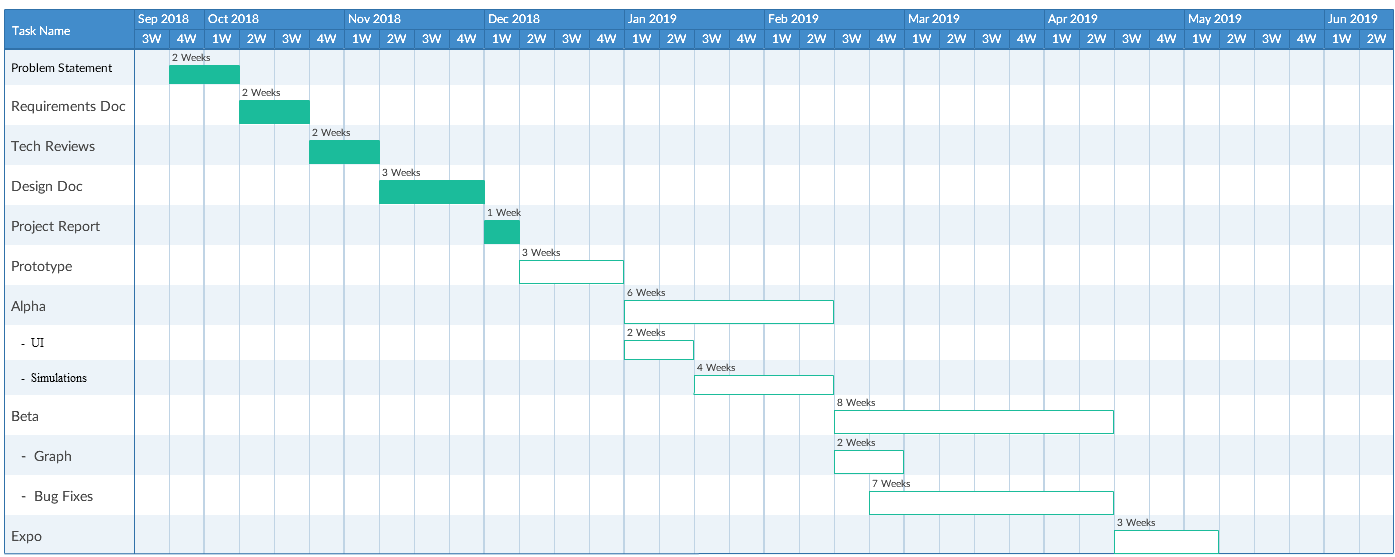
\includegraphics[width=\textwidth]{GanttChart1.png}

\section{Glossary}
\begin{enumerate}
    \item Inquiry-based learning - A form of learning that starts by posing questions rather than providing facts.
    \item IBLA - Inquiry based learning activity
    \item Parameter - a value is selected for the particular circumstances that affects the system. 

\end{enumerate}

\end{document}